\documentclass[a4paper,12pt]{report}

\usepackage{alltt, fancyvrb, url}
\usepackage{graphicx}
\usepackage[utf8]{inputenc}
\usepackage{float}
\usepackage{hyperref}
\usepackage{listings}
\usepackage{xcolor}

% Questo commentalo se vuoi scrivere in inglese.
\usepackage[italian]{babel}

\usepackage[italian]{cleveref}

% Definizione stili per blocchi di codice
\lstdefinelanguage{bash}{
    keywords={cd, ls, mv, cp, rm, mkdir, rmdir, echo, cat, sudo, git, python3, pip, docker, npm},
    sensitive=true,
    morecomment=[l]{\#},
    alsoletter={-}
}
\lstdefinestyle{bash}{
    language=bash,
    basicstyle=\ttfamily\small,
    backgroundcolor=\color{gray!10},
    frame=single,
    breaklines=true,
    keywordstyle=\color{blue},
    commentstyle=\color{gray}\itshape,
}
\lstdefinestyle{scala}{
    language=Scala,
    basicstyle=\ttfamily\small,
    backgroundcolor=\color{gray!10},
    frame=single,
    breaklines=true,
    keywordstyle=\color{blue},
    commentstyle=\color{gray}\itshape,
    stringstyle=\color{orange},
}

\title{Relazione Assignment-03 \\
1.About Asyncronous Message Passing with Actors (not distributed)\\ per l'esame \\ ``Programmazione Concorrente e Distribuita''}
\author{Giosuè Giocondo Mainardi}

\date{\today}

\begin{document}

\maketitle

\tableofcontents

\chapter{Analisi}
% A brief analsysis of the problem, focusing in particular aspects that are relevant from concurrent point of view.
    Il modello di simulazione dei Boid, formulato da Craig Reynolds nel 1986, rappresenta un sistema multi-agente in cui 
    entità autonome (Boid) si muovono in uno spazio condiviso, modificando la propria traiettoria in funzione dei Boid 
    circostanti e di parametri predefiniti.
    
    Dal punto di vista computazionale, l'algoritmo presenta una complessità computazionale di O(n²) nel caso peggiore, dove n rappresenta 
    il numero di Boid nella simulazione, dato che l'aggiornamento sincronizzato delle velocità di ciascun Boid avviene
    in base alle posizioni correnti dei vicini. Procede l'aggiornamento delle posizioni secondo le nuove velocità 
    calcolate, per poi infine renderizzare lo stato aggiornato tramite l'interfaccia grafica.
    
    In ottica di ottimizzazione delle prestazioni tramite programmazione concorrente, emerge l'opportunità di distribuire 
    il carico computazionale tra più unità di elaborazione. Tale distribuzione deve tuttavia preservare la correttezza 
    dell'algoritmo, garantendo che l'aggiornamento delle velocità preceda sempre quello delle posizioni, e che la 
    visualizzazione avvenga solo a computazione completata.

    Nel contesto dell'Asyncronous Message Passing con Attori, si propone di implementare un sistema in cui ogni Boid 
    è rappresentato da un attore autonomo, responsabile del proprio stato e della logica di aggiornamento.

    \section{Sfide della programmazione concorrente}
        L'implementazione concorrente della simulazione presenta diverse sfide specifiche che devono essere affrontate:

        \subsection*{Sincronizzazione delle fasi di calcolo}
            La natura sequenziale dell'algoritmo richiede una sincronizzazione rigorosa tra le fasi di:
            \begin{enumerate}
                \item Calcolo delle nuove velocità (basato sulle posizioni correnti)
                \item Aggiornamento delle posizioni (basato sulle nuove velocità)
                \item Rendering dell'interfaccia grafica
            \end{enumerate}
            
            Questa dipendenza temporale impedisce la sovrapposizione delle fasi e richiede punti di sincronizzazione 
            espliciti per garantire la correttezza dell'algoritmo.

        \subsection*{Condivisione dello stato}
            Tutti i Boid necessitano di accedere in lettura alle posizioni e velocità degli altri Boid durante il calcolo 
            delle proprie nuove velocità. Questo accesso concorrente in sola lettura non presenta problemi di race condition, 
            ma richiede meccanismi per garantire la consistenza dei dati visualizzati.

        \subsection*{Gestione delle risorse grafiche}
            L'interfaccia grafica rappresenta una risorsa condivisa che deve essere aggiornata in modo thread-safe. 
            La visualizzazione deve avvenire sul thread principale dell'interfaccia utente, richiedendo meccanismi 
            di comunicazione tra i thread di calcolo e quello di rendering.

    \section{Vantaggi del modello ad attori}
        L'adozione del modello ad attori per l'implementazione della simulazione offre diversi vantaggi significativi:

        \subsection*{Incapsulamento dello stato}
            Ogni Boid, rappresentato da un attore, mantiene il proprio stato interno (posizione, velocità) in modo 
            completamente isolato. Questo elimina i problemi di accesso concorrente allo stato condiviso e semplifica 
            notevolmente il reasoning sulla correttezza del sistema.

        \subsection*{Comunicazione asincrona}
            Il message passing asincrono consente una maggiore flessibilità nel scheduling delle operazioni e riduce 
            i problemi di deadlock tipici degli approcci basati su lock espliciti.

        \subsection*{Scalabilità}
            Il modello ad attori scala naturalmente con il numero di core disponibili, permettendo di sfruttare 
            efficacemente architetture multi-core e distribuire il carico computazionale.

        \subsection*{Fault tolerance}
            Gli attori possono essere supervisionati e riavviati in caso di errore, migliorando la robustezza 
            complessiva del sistema.


\chapter{Design}
% A description of the adopted design, the strategy and architecture.

    % Conversione in Scala
    L'applicazione è stata completamente convertita in \texttt{Scala}, partendo dal design già sviluppato per l'Assignment-01 e adottando uno stile funzionale e pulito.

    % Architettura generale
    Il design dell'applicazione si basa su un'architettura a tre livelli, ispirata al pattern Model-View-Controller (MVC).
    \begin{itemize}
        \item \texttt{BoidsModel}: gestisce lo stato della simulazione, inclusi i Boid e le loro proprietà.
        \item \texttt{BoidsView}: si occupa della visualizzazione grafica dei Boid e dell'interfaccia utente.
        \item \texttt{BoidsSimulator}: funge da intermediario tra Model e View, gestendo la logica di aggiornamento e le interazioni dell'utente.
    \end{itemize}

    % Utilizzo Akka e adozione FSM da Dining Hakkers
    È stato poi adottato il framework \texttt{Akka} per definire un'architettura orientata al message passing, scegliendo il modello \textbf{FSM}\footnote{\href{https://doc.akka.io/libraries/akka-core/current/typed/fsm.html}{Behaviors as finite state machines}}(Finite State Machines) proposto a lezione e ispirandosi all'esempio fornito dei \texttt{Dining Hakkers}\footnote{\href{https://github.com/cric96/pcd-lab-akka-actors/blob/63e4f3273ef1550c1c744d1f7332b7ce935223ab/src/main/scala/it/unibo/pcd/akka/basics/e07fsm/DiningHakkers.scala}{Adattamento da akka-samples by cric-96}}.
    
    % Spiegazione FSM
    Utilizzando il modello \textbf{FSM}, ogni attore può essere in uno stato specifico e rispondere a messaggi in modo differente a seconda dello stato corrente, definendo diversi  \texttt{Behavior}. Questo approccio consente di gestire la logica di controllo della simulazione in modo chiaro e modulare, facilitando l'estensione e la manutenzione del codice.

    % Dove viene usato il modello FSM?
    Questo stile è stato adottato in due aree precise dell'applicazione: nell'aggiornamento dei Boids da parte del Model e nel Loop di Controllo dell'applicazione
    
    \section{Loop di Controllo dell'applicazione}
        La comunicazione nel BoidsSimulator avviene tramite due protocolli distinti:
        \begin{itemize}
            \item \texttt{Update}: per far partire l'aggiornamento al Model con \texttt{Update.Boids}, il quale risponde con \texttt{Update.View} quando ha finito. 
            \item \texttt{UI}: per la gestione dell'interfaccia utente, comprende i comandi \texttt{Start}, \texttt{Stop}, \texttt{Pause}, \texttt{Resume} e \texttt{ChangeAttribute}.
        \end{itemize}

        Entrambi i protocolli estendono il trait \texttt{Loop}, garantendo un'interfaccia uniforme per la gestione dei messaggi.

        Gli stati modellati nel \texttt{BoidsSimulator} sono:
        \begin{itemize}
            \item \texttt{notRunning}: lo stato iniziale.
            \item \texttt{running}: quando la simulazione è attiva e i Boids vengono aggiornati.
            \item \texttt{suspended}: quando la simulazione è sospesa, ma può essere ripresa.
            \item \texttt{start}: quando la simulazione può essere avviata correttamente.
        \end{itemize}

        Con due stati ausiliari:
        \begin{itemize}
            \item \texttt{handleAttributeChanging}: quando viene cambiato un attributo dagli sliders.
            \item \texttt{updateBoids}(solo per lo stato \texttt{running}): per creare un attore dal Model e delegarlo dell'aggiornamento dei Boids.
        \end{itemize}
        
    \section{Aggiornamento dei Boids}
        Nell'implementazione scelta un Boid ora è semplicemente un oggetto con posizione e velocità accessibili e modificabili (getter/setter), mentre della logica di aggiornamento se ne occupa una classe separata \texttt{BoidActor}, che wrappa il Boid.
        Ogni Boid è quindi rappresentato da un attore autonomo responsabile del proprio stato e dei calcoli necessari. I \texttt{BoidActor} comunicano con il Model esclusivamente attraverso messaggi asincroni, garantendo una gestione naturale della concorrenza e una chiara separazione delle responsabilità.

        \subsection*{BoidsModel}
            Il ciclo di aggiornamento dei Boids è orchestrato da un attore principale \texttt{BoidsModel}, avviato dal Controller, che coordina le operazioni e può ricevere solo due semplici comandi (dai \texttt{BoidActor}):
            \begin{itemize}
                \item \texttt{UpdatedBoidsVel}
                \item \texttt{UpdatedBoidsPos}
            \end{itemize}
            Tramite questi può tenere traccia del numero di Boid che hanno aggiornato la propria velocità e posizione, rispettivamente.
        
        \subsection*{BoidActor}
            D'altra parte, il Model può mandare ai \texttt{BoidActor} uno dei seguenti messaggi:
            \begin{itemize}
                \item \texttt{UpdateVel}: per calcolare la nuova velocità in base alle regole di interazione con i Boids vicini.
                \item \texttt{UpdatePos}: per aggiornare la posizione in base alla velocità corrente.
                \item \texttt{Kill}: per terminare l'attore Boid.
            \end{itemize}
        
\chapter{Comportamento}
% A description of the behaviour of the system using one or multiple Petri Nets, choosing the propor level of abstraction.
    % Introduzione alle reti di Petri
    Il comportamento del sistema di simulazione dei Boid viene formalizzato attraverso reti di Petri che catturano gli aspetti dinamici e la sincronizzazione tra i diversi componenti. Questo modello formale permette di rappresentare efficacemente sia l'interazione dell'utente con l'applicazione che il ciclo di aggiornamento interno della simulazione.

    Inoltre, avendo adottato il modello \textbf{FSM}, vengono forniti anche dei piccoli automi che rappresentano gli attori modellati, per evidenziare i loro possibili stati e messaggi accettabili.
    
    \section{Loop di Controllo dell'applicazione}
        Una volta inizializzata l'applicazione con un numero specificato di Boid, l'utente può avviare la simulazione tramite il comando \texttt{start}. Durante l'esecuzione, è possibile fermarne completamente il funzionamento con \texttt{stop} (che riporta il sistema allo stato iniziale liberando tutte le risorse), oppure metterla temporaneamente in pausa con \texttt{suspend} per poi riprenderla successivamente con \texttt{resume}.

        \subsection*{Rete di Petri}
            Nella rete in Fig. \ref{fig:rete_app_flow} vengono rappresentati gli stati come piazze e i messaggi come transizioni. Più precisamente, le transizioni marchiate con \textbf{UI} (User Interaction) rappresentano i comandi dell'utente, mentre le altre (che iniziano con \textbf{Update}) rappresentano le interazioni dell'aggiornamento con il Model.
            \begin{figure}[ht!]
                \centering
                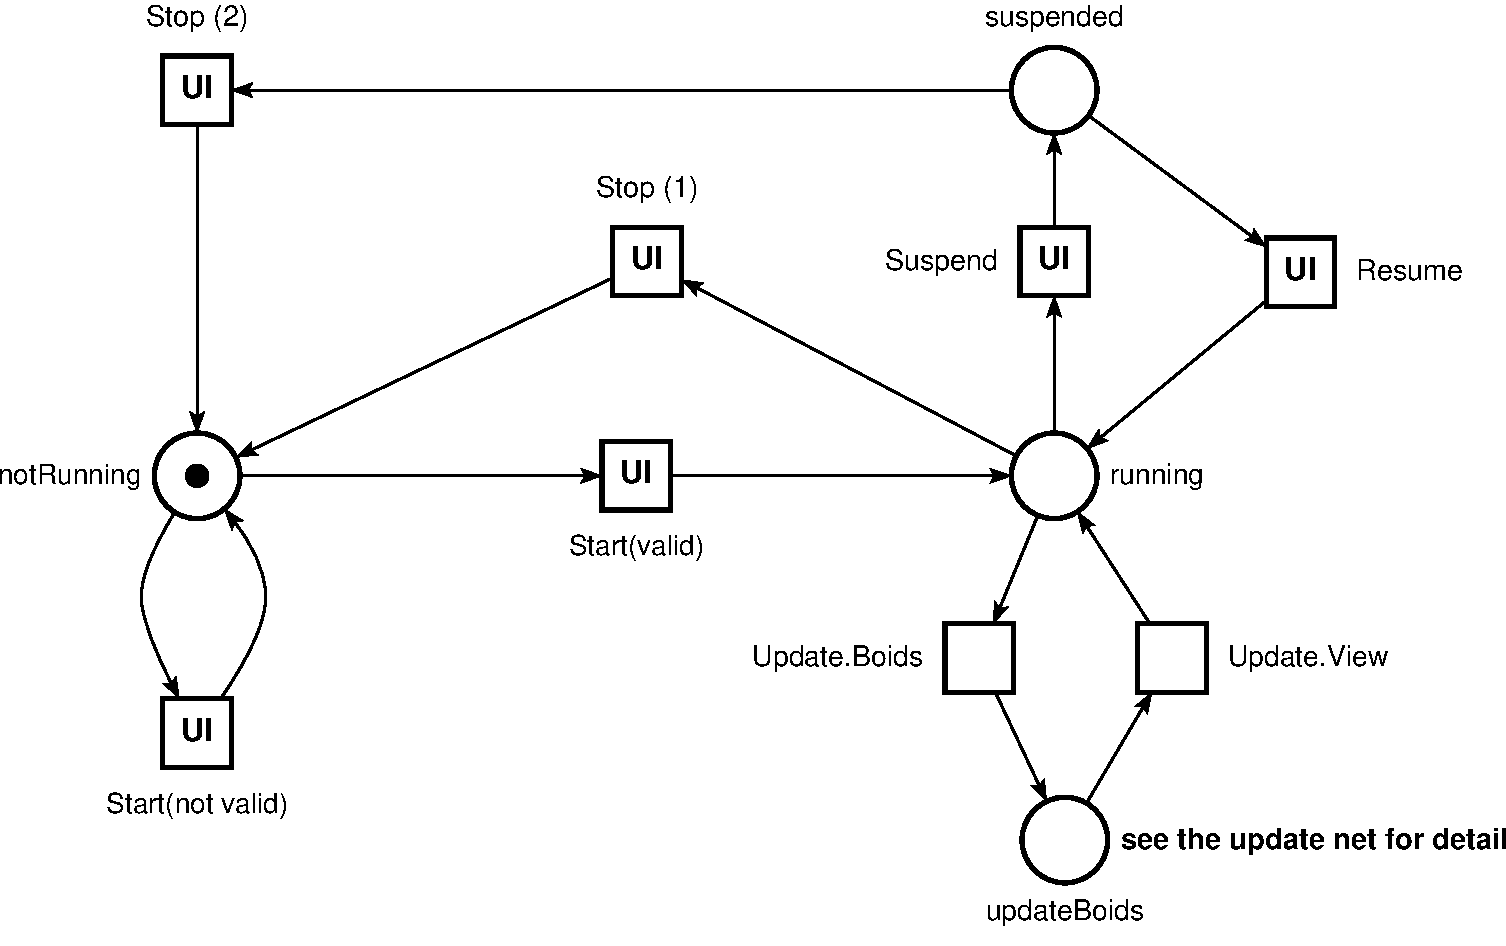
\includegraphics[width=0.8\textwidth]{petri_nets_pdf/rete_app_flow.pdf}
                \caption{Rete di Petri per il flusso di esecuzione con input dell'utente.}
                \label{fig:rete_app_flow}
            \end{figure}
            
            Per chiarire il comportamento del comando di stop, è importante sottolineare che questo evento termina tutti i \texttt{BoidActor}, senza attendere il completamento del ciclo di calcolo corrente. Questo comportamento è intenzionale e riflette l'implementazione del sistema, dove il comando di stop ha priorità assoluta e causa la terminazione immediata degli attori figli, indipendentemente dal loro stato di avanzamento nel ciclo di calcolo.

        \subsection*{Automa a stati finiti}
            Gli stati modellati nel \texttt{BoidsSimulator} e i possibili messaggi accettati sono rappresentati dall'automa a stati finiti in figura:
            \begin{figure}[ht!]
                \centering
                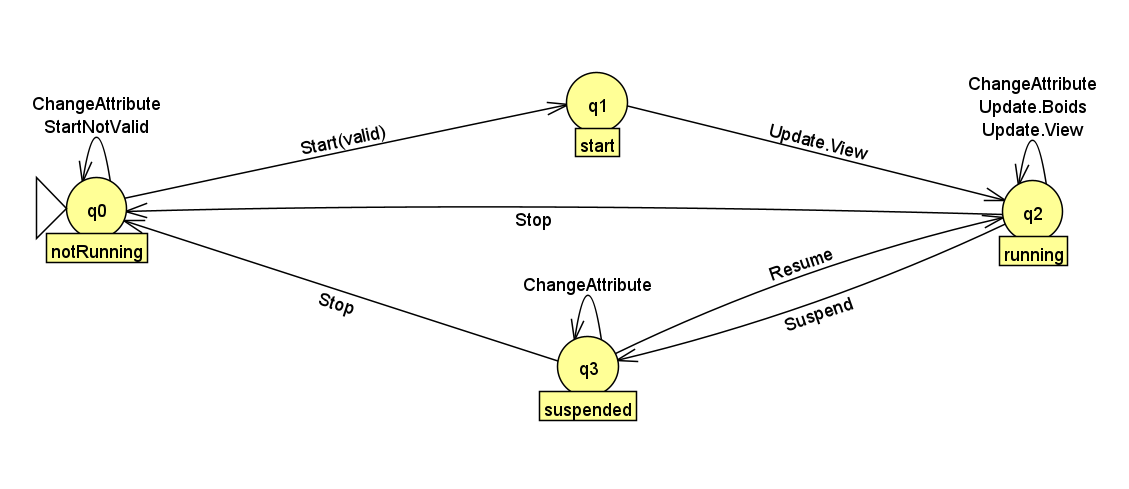
\includegraphics[width=\textwidth]{img/FSM/Simulator.png}
                \caption{Automa a stati finiti del BoidsSimulator.}
                \label{fig:Boids_simulator_fsm}
            \end{figure}
    
    \section{Aggiornamento dei Boids}
        %ciclo di aggiornamento della simulazione, mostrando le dipendenze tra il calcolo delle velocità e l'aggiornamento delle posizioni, nonché i punti di sincronizzazione necessari per mantenere la coerenza del modello.

        Il ciclo di aggiornamento della simulazione nel Model inizia con lo stato iniziale \texttt{updateBoids}, creato dal Controller, questo passa direttamente allo stato \texttt{startUpdatingVel} che chiede a tutti i Boid di calcolare la propria velocità e si mette in attesa di risposta in \texttt{updatingVel}. Una volta che tutti i Boid hanno risposto, il Model passa allo stato \texttt{startUpdatingPos} per aggiornare le posizioni dei Boid, attende in \texttt{updatingPos} fino a quando tutti i Boid hanno aggiornato le loro posizioni. 
        Infine, dopo aver ricevuto tutte le risposte, il Model passa allo stato \texttt{endUpdatingPos} che dice al Controller di aggiornare la View, poi termina.
        
        
        \subsection*{Rete di Petri}
            \begin{figure}[ht!]
                \centering
                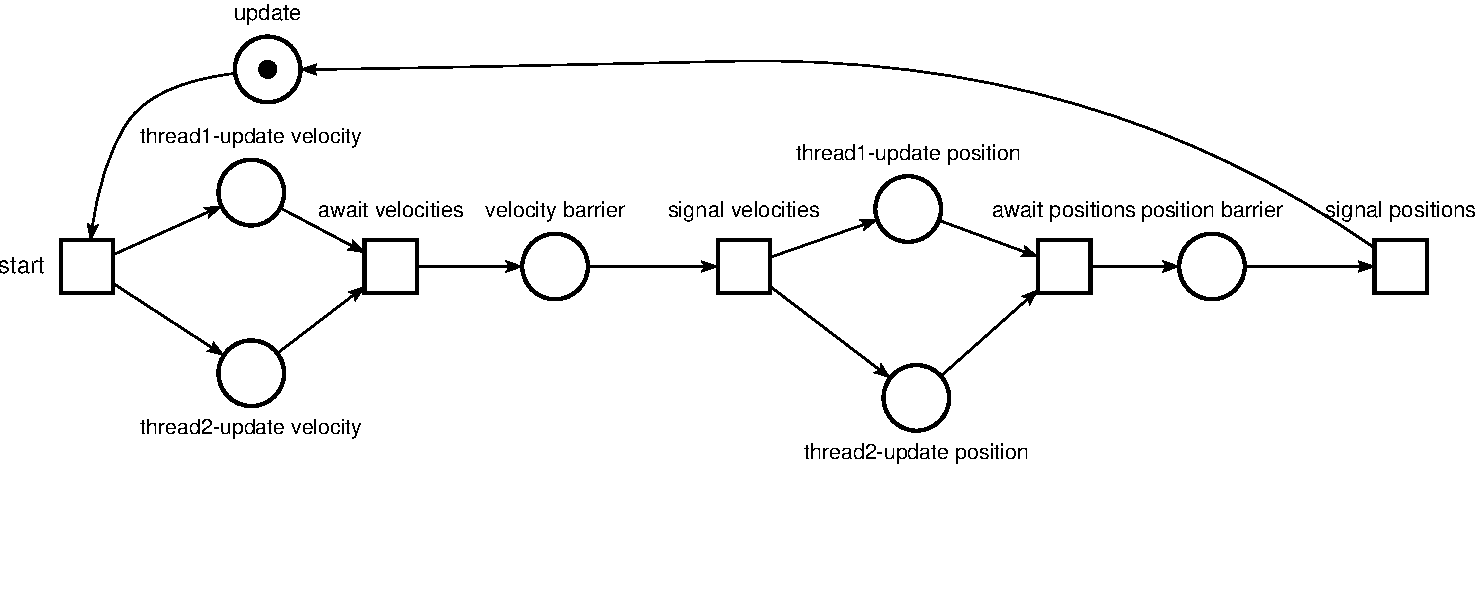
\includegraphics[width=\textwidth]{petri_nets_pdf/rete_update_cycle.pdf}
                \caption{Rete di Petri per il ciclo di aggiornamento della simulazione.}
                \label{fig:rete_update_cycle}
            \end{figure}

            La rete in Fig. \ref{fig:rete_update_cycle} evidenzia chiaramente i punti di sincronizzazione necessari per mantenere la coerenza del modello, garantendo che le operazioni di calcolo delle velocità e aggiornamento delle posizioni siano eseguite in modo sequenziale e coordinato tra i vari BoidActors.

        \subsection*{Automa a stati finiti dell'aggiornamento}
            Per migliorare la comprensione del ciclo di aggiornamento della simulazione, è stato creato un automa a stati finiti (FSM) che rappresenta il comportamento del Model. Questo automa mostra gli stati principali e le transizioni tra di essi, modellati con messaggi.

            \begin{figure}[ht!]
                \centering
                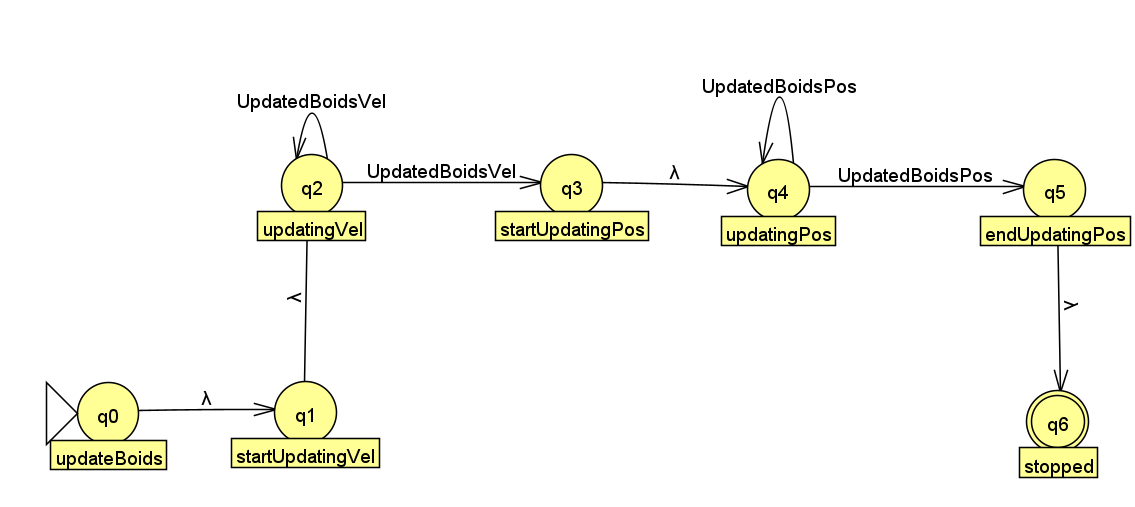
\includegraphics[width=\textwidth]{img/FSM/BoidsModel.png}
                \caption{Automa a stati finiti dell'updateBoids nel Model.}
                \label{fig:Boids_model_fsm}
            \end{figure}
        \subsection*{Automa a stati finiti del BoidActor}
            Ogni BoidActor può aggiornare il suo stato tramite i messaggi \texttt{UpdateVel} e \texttt{UpdatePos}, oppure terminare la propria esecuzione con il messaggio \texttt{Kill}. Questi messaggi sono gestiti in modo asincrono, consentendo a ciascun BoidActor di operare in parallelo con gli altri.

            Il suo automa può essere rappresentato come in figura:
            \begin{figure}[ht!]
                \centering
                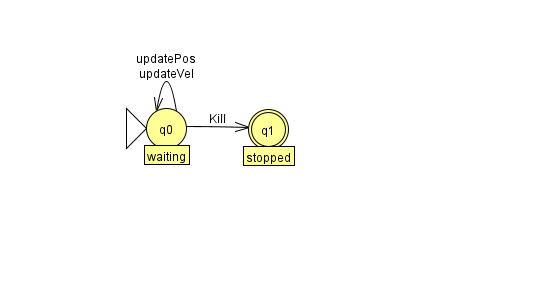
\includegraphics[width=\textwidth]{img/FSM/BoidActor.png}
                \caption{Automa a stati finiti del BoidActor.}
                \label{fig:Boid_actor_fsm}
            \end{figure}

        \begin{lstlisting}[style=bash, caption={Avvio dello script}]
            $ mvn clean javafx:run
        \end{lstlisting}
    
    
\end{document}
